%**************************************************************************
%* SpringSim 2017 Author Kit
%*
%* Word Processing System: TeXnicCenter and MiKTeX
%*
%**************************************************************************

\documentclass{scspaperproc}

\usepackage{latexsym}
\usepackage{graphicx}
\usepackage{mathptmx}
\usepackage{amsmath}
\usepackage{amsfonts}
\usepackage{amssymb}
\usepackage{amsbsy}
\usepackage{amsthm}
%\usepackage[pdftex,colorlinks=true,urlcolor=blue,citecolor=black,anchorcolor=black,linkcolor=black]{hyperref}
%% \usepackage[dvips,colorlinks=true,urlcolor=blue,citecolor=black,%
%% anchorcolor=black,linkcolor=black]{hyperref}

% custom hyphenation rules
\usepackage{hyphenat}
\hyphenation{op-tical net-works semi-conduc-tor}

% theorem style
\newtheoremstyle{scsthe}% hnamei
{8pt}% hSpace abovei
{8pt}% hSpace belowi
{\it}% hBody fonti
{}% hIndent amounti1
{\bf}% hTheorem head fontbf
{.}% hPunctuation after theorem headi
{.5em}% hSpace after theorem headi2
{}% hTheorem head spec (can be left empty, meaning `normal')i
\theoremstyle{scsthe}
\newtheorem{theorem}{Theorem}
\renewcommand{\thetheorem}{\arabic{theorem}}
\newtheorem{corollary}[theorem]{Corollary}
\renewcommand{\thecorollary}{\arabic{corollary}}
\newtheorem{definition}{Definition}
\renewcommand{\thedefinition}{\arabic{definition}}

% avoid overrunning the right margin
\sloppy

%% ***** NOTE *****

%% The use of the long citation format (e.g. "Brown and Edwards
%% (1993)" rather than "[5]") and at the same time using the hyperref
%% package can lead to hard to trace bugs in case the citation is
%% broken accross the line (usually this will mark the entire
%% paragraph as a hyperlink (clickable) which is easily noticeable and
%% fixed if using colorlinks, but not if the color is black -- as it
%% is now). Worse yet, if a citation spans page boundary, LaTeX
%% compilation can fail, with an obscure error message. Since this
%% depends a lot on the flow of the text and wording, these bugs come
%% and go and can be extremely hard for a beginner to trace. The error
%% message can look like this:
%%
%%    ! pdfTeX error (ext4): \pdfendlink ended up in different nesting
%%    level than \pdfstartlink.  \AtBegShi@Output ...ipout \box
%%    \AtBeginShipoutBox \fi \fi
%%    l.174 
%%    ! ==> Fatal error occurred, no output PDF file produced!
%%
%% and can be universally fixed by putting an \mbox{} around the
%% citation in question (in this case, at line 174) and maybe adapting
%% the wording a little bit to improve the paragraph typesetting,
%% which is perhaps not immediately obvious.
%****************************************************************************

% begin document
\begin{document}

% Page header (author list)
\SCSpagesetup{Lux, Watson, Chang, Bernard, Li, Xu, Back, Butt, Cameron, and Hong}

% Conference info
\def\SCSconferenceacro{SpringSim}
\def\SCSpublicationyear{2018}
\def\SCSconferencedates{April 15-18}
\def\SCSconferencevenue{Baltimore, MD, USA}
\def\SCSsymposiumacro{HPC} % High Performance Computing Symposium

% title
\title{Predictive Modeling of I/O Characteristics \\ in High
  Performance Computing Systems}

% AUTHOR LIST
% *** NOTE: May need to adjust titlevboxsize in the preamble
\author{Thomas C. H. Lux \\ [12pt]
Dept. of Computer Science \\
Virginia Polytechnic Institute\\
\& State University \\
Blacksburg, VA 24061 \\
tchlux@vt.edu \\
\and
Layne T. Watson \\[12pt]
Dept. of Computer Science\\
Dept. of Mathematics\\
Dept. of Aerospace \& Ocean Eng.\\ 
Virginia Polytechnic Institute\\
\& State University \\
\and
Tyler H. Chang\\
Jon Bernard\\
Bo Li\\[12pt]
Dept. of Computer Science\\ 
Virginia Polytechnic Institute\\
\& State University \\
\and
Li Xu\\[12pt]
Dept. of Statistics\\ 
Virginia Polytechnic Institute\\
\& State University \\
\and
Godmar Back\\
Ali R. Butt\\
Kirk W. Cameron\\[12pt]
Dept. of Computer Science\\ 
Virginia Polytechnic Institute\\
\& State University \\
\and
Yili Hong\\[12pt]
Dept. of Statistics\\ 
Virginia Polytechnic Institute\\
\& State University \\
}

\maketitle

\section*{Abstract}

Each of high performance computing, cloud computing, and computer
security have their own interests in modeling and predicting the
performance of computers with respect to how they are configured. An
effective model might infer internal mechanics, minimize power
consumption, or maximize computational throughput of a given
system. This paper analyzes a four-dimensional dataset measuring the
input/output (I/O) characteristics of a cluster of identical computers
using the benchmark IOzone. The I/O performance characteristics are
modeled with respect to system configuration using multivariate
interpolation and approximation techniques. The analysis reveals that
accurate models of I/O characteristics for a computer system may be
created from a small fraction of possible configurations, and that
some modeling techniques will continue to perform well as the number
of system parameters being modeled increases. These results have
strong implications for future predictive analyses based on more
comprehensive sets of system parameters.

\textbf{Keywords:} Regression, approximation, interpolation,
performance modeling


%     Introduction     
%======================
\section{Introduction}

Performance tuning is often an experimentally complex and time-intense
chore necessary for configuring HPC systems. The procedures for this
tuning vary largely from system to system and are often subjectively
guided by the system engineer(s). Once a desired level of performance
is achieved, an HPC system may only be incremenetally reconfigured as
required by updates or specific jobs. In the case that a system has
changing workloads or non-stationary performance objectives that range
from maximizing computational throughput to minimizing power
consumption and system variability, it becomes clear that a more
effective and automated tool is needed for configuring systems. This
scenario presents a challenging and important application of
multivariate approximation and interpolation techniques.

Predicting the performance of an HPC system is a challenging problem
that is primarily attempted in one of two ways: (1) build a
statistical model of the performance by running experiments on the
system at select settings or (2) use a performance simulator to run
artificial experiments and search for optimal configurations. In this
paper the proposed multivariate modelling techniques rest in the first
category, however they represent a notable increase in the ability to
model more complex interactions between system parameters.

Many previous works attempting to model system performance have used
simulated environments to estimate the performance of a
system. \cite{grobelny2007fase,wang2009simulation,wang2013towards}
Some of these works cite statistical models as being over-simplified
and not capabel of capturing the true complexity of the underlying
system. This claim is partially correct, noting that a large portion
of predictive statistical models rely on simplifying the system to one
or two parameters.
\cite{snavely2002framework,bailey2005performance,barker2009using,ye2010analyzing}
These limited statistical models have provided satisfactory
performance in very narrow application settings. Many of the
aforementioned statistical modeling techniques claim to generalize,
while simultaneously requiring additional code annotations, hardware
abstractions, or additional application level understandings in order
to generate models. The approach presented here requires no
modifications of the application, no architecture abstractions, nor
any structural descriptions of the input data being modelled. The
techniques used are purely mathematical and only need formatted data
as input.

Among the statistcal models presented in prior works,
\cite{bailey2005performance} specifically mentions that it is
difficult for the simplified models to capture variability introduced
by I/O. System variability in general has become a problem of
increasing interest to the HPC and systems communities, however most
of the work has focused on Operating System (OS) induced variability.
\cite{beckman2008benchmarking,de2007identifying} The work that
has focused on managing I/O variability, \cite{lofstead2010managing},
does not use any sophisticated modeling techniques. Hence, this paper
presents a case study applying advanced mathematical and statistical
modeling techniques to the domain of HPC I/O characteristics. The
models are used to predict the mean throughput of a system and the
variance in throughput of a system. The discussion section outlines
how the exact techniques presented can be applied to any performance
metric and any system.

%% Multivariate models for an HPC system would be a function of the
%% tunable parameters built to accurately model some desired performance
%% metric.

%% \begin{enumerate}
%% \item The value of multivariate Modeling
%% \item The data context
%% \item The proposed method for using multivariate models
%% \item The impact of effective models
%% \end{enumerate}

In general, this paper compares five multivariate approximation
techniques that operate on inputs in $\mathbb{R}^d$ (vectors of $d$
real numbers) and produce predicted responses in $\mathbb{R}$. In
order to provide coverage of the varied mathematical strategies that
can be employed to solve the continuous modeling problem, three of the
techniques are regression-based and the remaining two techniques
produce interpolants. The sections below outline the mathematical
formulations of each technique and provide computational complexity
bounds with respect to the size (number of points and dimension) of
input data. Throughout the sections, $d$ will refer to the dimension
of the input data, $n$ is the number of points in the input data,
$x_i \in \mathbb{R}^d$ is the $i^{th}$ input data point, and $y_i$ is
the response value of the $i^{th}$ input data point.

\subsection{Approximation}
Multivariate approximations are capable of accurately modelling
complex relationships between the dimensions of any set of points in
$\mathbb{R}^d$ with respect to some response in $\mathbb{R}$. The
approximations produce a function $f: \mathbb{R}^d \rightarrow
\mathbb{R}$ which minimizes some selected error metric related to the
provided data. Often, as in least-squares regression, the distance
metric chosen is the sum of squared differences between modeled
response values and true response values.

\subsubsection{Multivariate Adaptive Regression Splines}
This algorithm was introduced by statistician J. Friedman in
\cite{friedman1991multivariate} and subsequently improved to it's
current version in \cite{stanford1993fast}. This work uses the Fast
Multivariate Adaptive Regression Splines (Fast MARS) formulation. In
Fast MARS, a least-squares fit model is iteratively built by beginning
with a single constant valued function and adding two new basis
functions at each iteration of the form

$$ B_{2s-1}(x) = B_l(x) [c(x_i-v)]_+ $$
$$ B_{2s}(x) = B_k(x) [c(x_i-v)]_- $$

Where $s$ is the iteration number, $B_l(x)$ and $B_k(x)$ are some
previously generated basis functions, $c, v \in \mathbb{R}$, and $x_i$
with $0 < i \leq d$ is the $i^{th}$ component (1 indexed) of input
vector $x$. After iteratively constructing a model, MARS then
iteratively removes basis functions that do not contribute to goodness
of fit. In effect, MARS creates a locally component-wise linear
approximation of the data that is $C^0$. The overall computational
complexity of Fast MARS is $\mathcal{O}(n d m^3)$ where $m$ is a user
selected value that is the maximum complexity of the model in terms of
the number of underlying basis functions. This paper uses an Earth
implementation of MARS \cite{rudy2017pyearth} with a max number of
basis functions of $n$, however with larger datasets ($n > 1000$) this
value would need to be reduced.

\subsubsection{Multi-Layer Perceptron Regressor}
The neural network is a well studied and widely used mathematical tool
for both regression and classification tasks.
\cite{hornik1989multilayer} When using the rectified linear unit
(ReLU) activation functions \cite{dahl2013improving} and trained using
the BFGS technique \cite{moller1993scaled}, the model built by a
multi-layer perceptron uses layers of the form

$$l(x) : \mathbb{R}^{i} \rightarrow \mathbb{R}^{j} = \text{max}\big( x
W_l, 0 \big)$$

Where $W_l$ is the $i$ by $j$ weight matrix of layer $l$ and the max
function is applied element-wise to the resulting vector. In this
form, the multi-layer perceptron (MLP) produces a locally linear model
of the input data that is $C^0$. The computational complexity of
training a multi-layer perceptron is approximately $\mathcal{O}(n d
m)$ where $m$ is a constant determined by a linear function of the
sizes of the layers of the network and the convergence stopping
criteria of the BFGS minimization used for finding weights. This paper
uses the scikit-learn MLP regressor \cite{scikit-learn} with a single
hidden layer with 100 nodes, ReLU activation, and BFGS for training.

\subsubsection{Support Vector Regressor}
Support vector machines are a common tool used in machine learning
classification tasks that can be adapted for the purpose of regression
\cite{basak2007support}. The mathematical formalisms for exactly how
to build a support vector regressor (SVR) are beyond the scope of this
summary, but the resulting functional fit is of the form

$$ f(x) : \mathbb{R}^d \rightarrow \mathbb{R} = \sum_{i=1}^{n}a_i
K(x,x_i) $$


%% $$ \text{Minimize } \bigg\{ \frac{1}{2}\sum_{i=1}^{n}\sum_{j=1}^{n}
%% a_i a_j K(x_i, x_j) + \epsilon \sum_{i=1}^{n} a_i - \sum_{i=1}^{n} y_i
%% a_i \bigg\} $$

%% $$ \text{Subject to } \sum_{i=1}^{n}a_i = 0 \text{ } \text{ and }
%% \text{ } a_i \in [0,C] $$

Where $K$ is the selected kernel function, $a \in \mathbb{R}^n$ is the
solved coefficient vector, and $\epsilon$ is the error tolerance. The
SVR is always fitting a linear function, however the kernel mapping of
the data can be non-linear to create non-linear fits. The
computational complexity of the SVR minimization (for the
implementation used) is $\mathcal{O}(n^2dm)$ with $m$ being a constant
determined by the minimization convergence criteria. This paper uses
the scikit-learn SVR \cite{scikit-learn} with a polynomial kernel
function.

\subsection{Interpolation}


\subsubsection{Delaunay}
\subsubsection{Linear Shepard}

The remainder of the paper is broken up into \_ parts. \textit{(will
  fill in the parts and descriptions once they are finalized)}

%% %     Related Work     
%% %======================
%% \section{Related Work}
%% \begin{enumerate}
%% \item Not sure how much to include here? Shooting for thoroughness or
%%   simply necessary coverage? How much background should I expect the
%%   readers of this paper to have in the ``multivariate modeling of
%%   systems'' area?
%% \end{enumerate}


%     Methodology     
%=====================
\section{Methodology}
\subsection{Data}
The summary of the data used in the experiments for this paper can be
seen in Table \ref{tab:data_type}.

\begin{table}
  \centering
  \begin{tabular}{|c|c|c|}
    \hline
    \textbf{System Parameter} & \textbf{Type} & \textbf{Values}\\
    \hline
    Hypervisor Scheduler & Categorical & CFQ, NOOP, DEAD\\
    Operating System Scheduler & Categorical & CFQ, NOOP, DEAD\\
    IOZone Test Type & Categorical & Fread, Fwrite, RandomRead\\
    File Size & Continuous & 64, 128, 256, 512, 1024\\
    Record Size & Continuous & 32 64, 128, 256, 512\\
    Thread Count & Continuous & 1,2,4,8,16,32,64\\
    Frequency & Continuous & 2.4, 2.5, 2.6, 2.7, 2.8, 2.9, 3.0, 3.1\\
    \hline
  \end{tabular}
  \caption{A description of the system parameters being considered in
    the IOZone tests. There are three categorical settings and four
    continuous settings. Notice that the ranges of values for
    continuous settings are different.}
  \label{tab:data_type}
\end{table}

\subsection{Dimensional Analysis}
This work utilizes an extension to standard k-fold cross validation
that allows for a more thorough investigation of the expected model
performance in a variety of real-world situations. Alongside
randomized splits, two extra components are considered: the amount of
training data provided, and the dimension of the input data. It is
important to consider that algorithms which perform well with less
training input also require less experimentation. Although, the amount
of training data required may change as a function of the number of
input dimensions and this needs to be studied as well.

The framework used in this paper will be referred to as a
multi-dimensional analysis (MDA) of the IOZone data presented in this
study. However, the MDA framework can be applied to other datasets.

\begin{enumerate}
\item Cycling the categorical settings
\item Selecting subsets of 1,2,3 up to 4 dimensions
\item Cycling different training : testing ratios (5:95 $\rightarrow$ 95:5)
\item Generating 200 random training : testing splits
\item Ensuring the testing points are on/inside the convex hull of the training.
\item Ensuring the training points are well-spaced.
\end{enumerate}

\subsection{Prediction}
\begin{enumerate}
\item For each file generated from the dimensional analysis, train on
  the training data, evaluate at the testing data points
\end{enumerate}


%     Results     
%=================
\section{Results}
\subsection{I/O Throughput Mean}

%% \begin{center}
%%   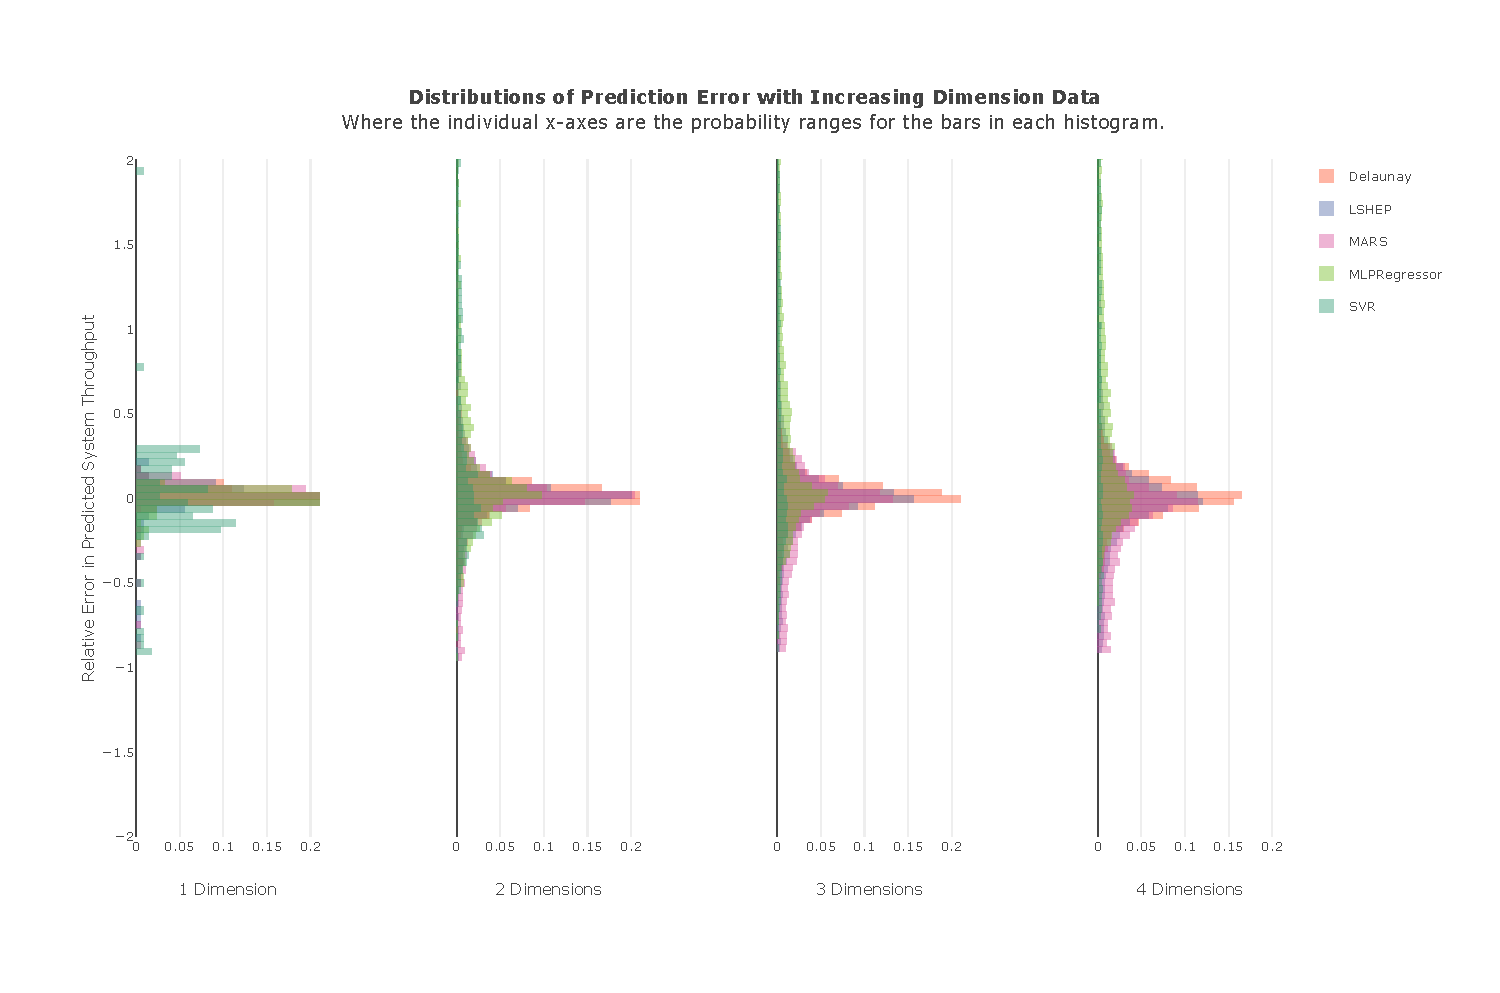
\includegraphics[width=\textwidth]{Prediction_Performance_Dim.pdf}
%%   \caption{In this figure we see how the distribution of errors }
%% \end{center}

\begin{figure}
  \centering
  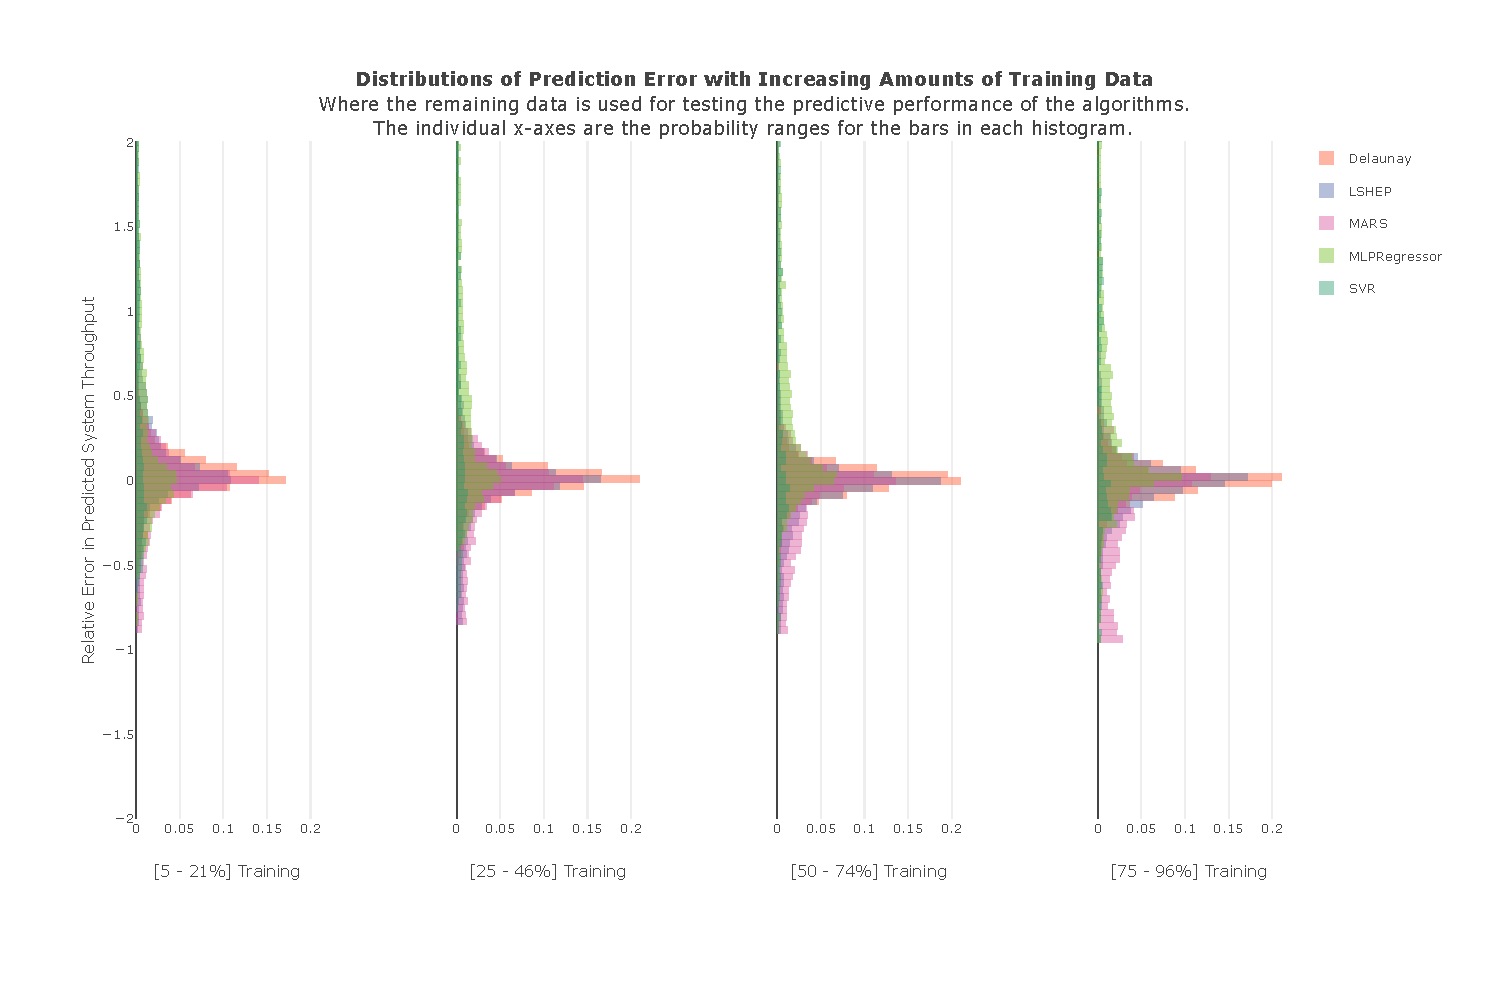
\includegraphics[width=\textwidth]{Prediction_Performance_TT_Ratio.pdf}
  \caption{In this figure, it can be seen how the distribution of
    prediction errors for each algorithm is affected by the quantity
    of training data provided. Notice that for all amounts of training
    data, Delaunay has the largest likelihoods around 0 error.}
  \label{fig:tt_ratio}
\end{figure}

\begin{table}
  \centering
  \begin{tabular}{|c||c|c|c|}
    %% \hline
    %% \multicolumn{4}{|c|}{Table Title}\\
    \hline
    \textbf{Algorithm} & \textbf{Input Dimension} & \textbf{Mean Absolute Error} & \textbf{Mean Relative Error}\\
    \hline
    Delaunay     & 1 & 2060267   & 0.03 \\
                 & 2 & 2916224   & 0.07 \\
                 & 3 & 3001794   & 0.09 \\
                 & 4 & 3134779   & 0.10 \\
    \hline
    LSHEP        & 1 & 6353148   & 0.06 \\
                 & 2 & 13038882  & 1.52 \\
                 & 3 & 5446207   & 1.13 \\
                 & 4 & 5133648   & 1.07 \\
    \hline
    MARS         & 1 & 2176368   & 0.03 \\
                 & 2 & 6213369   & 0.61 \\
                 & 3 & 4024964   & 0.65 \\
                 & 4 & 4497414   & 1.01 \\
    \hline
    MLPRegressor & 1 & 2461097   & 0.06 \\
                 & 2 & 8883580   & 0.81 \\
                 & 3 & 11190977  & 2.03 \\
                 & 4 & 11831721  & 2.20 \\
    \hline
    SVR          & 1 & 19306731  & 0.96 \\
                 & 2 & 78213963  & 18.49\\
                 & 3 & 97761266  & 31.27\\
                 & 4 & 113551300 & 37.2 \\
    \hline
  \end{tabular}
  \caption{Most models experience a decay in predictive performance as
    the dimension of the data increases. This is expected because
    higher dimension input has exponentially more possible patterns to
    identify. The MLP Regressor and SVR experience the worst decay in
    performance with increasing dimension.}
  \label{tab:perf_by_dim}
\end{table}

\begin{table}
  \centering
  \begin{tabular}{|c||c|c|c|}
    %% \hline
    %% \multicolumn{4}{|c|}{Table Title}\\
    \hline
    \textbf{Algorithm} & \textbf{Training Data} & \textbf{Mean Absolute Error} & \textbf{Mean Relative Error}\\
    \hline
    Delaunay     & [5-21]\%  & 5274933   & 0.11 \\
                 & [25-46]\% & 2898330   & 0.08 \\
                 & [50-74]\% & 1518477   & 0.07 \\
                 & [75-96]\% & 886346    & 0.08 \\
    \hline
    LSHEP        & [5-21]\%  & 13218469  & 2.53 \\
                 & [25-46]\% & 4936381   & 0.85 \\
                 & [50-74]\% & 2251409   & 0.26 \\
                 & [75-96]\% & 1415034   & 0.15 \\
    \hline
    MARS         & [5-21]\%  & 6543153   & 0.61 \\
                 & [25-46]\% & 4324916   & 0.80 \\
                 & [50-74]\% & 3115943   & 0.95 \\
                 & [75-96]\% & 2591451   & 0.74 \\
    \hline
    MLPRegressor & [5-21]\%  & 17348982  & 2.58 \\
                 & [25-46]\% & 12504957  & 2.29 \\
                 & [50-74]\% & 5292177   & 1.17 \\
                 & [75-96]\% & 2996253   & 1.02 \\
    \hline
    SVR          & [5-21]\%  & 170906944 & 49.45\\
                 & [25-46]\% & 99851846  & 31.28\\
                 & [50-74]\% & 51565405  & 19.63\\
                 & [75-96]\% & 27125130  & 12.6 \\
    \hline
  \end{tabular}
  \caption{All models experience a reduction in error with increasing
    amounts of training data. This suggests that the data being
    modeled is pattern-dense, over-fitting is \textit{not} occurring,
    and that oversimplifications will tend towards worse predictions.}
  \label{tab:perf_by_tt}
\end{table}

\subsection{I/O Throughput Variance}
\subsection{Increasing Dimension}


%     Discussion     
%====================
\section{Discussion}
\subsection{Modeling the System}
\subsection{Quantifying Variability}
\subsection{Extending the Analysis}

%     Future Work     
%=====================
\section{Future Work}
The most severe limitation to the presented work is the present
inability to model the relationship between categorical system
parameters. This could be seen as a limitation of the models selected,
because only MARS is capable of handling non-numeric variables, or as
a limitation of the MDA framework.


\bibliographystyle{scsproc}
\bibliography{paper}

\end{document}


%%  ALGORITHM     MEAN ABSOLUTE ERROR    MEAN RELATIVE ERROR
                                                      
%% 1 Dimension                                        
%%  Delaunay         2060267             0.03 
%%  MARS             2176368             0.03 
%%  MLPRegressor     2461097             0.06 
%%  LSHEP            6353148             0.06 
%%  SVR             19306731             0.96 
                                                      
%% 2 Dimensions                                       
%%  Delaunay         2916224             0.07 
%%  MARS             6213369             0.61 
%%  MLPRegressor     8883580             0.81 
%%  LSHEP           13038882             1.52 
%%  SVR             78213963             18.49
                                                      
%% 3 Dimensions                                       
%%  Delaunay         3001794             0.09 
%%  MARS             4024964             0.65 
%%  LSHEP            5446207             1.13 
%%  MLPRegressor    11190977             2.03 
%%  SVR             97761266             31.27
                                                      
%% 4 Dimensions                                       
%%  Delaunay         3134779             0.10 
%%  MARS             4497414             1.01 
%%  LSHEP            5133648             1.07 
%%  MLPRegressor    11831721             2.20 
%%  SVR            113551300             37.26
                                                      
%% [5 - 21%] Training Data               
%%  Delaunay         5274933             0.11 
%%  MARS             6543153             0.61 
%%  LSHEP           13218469             2.53 
%%  MLPRegressor    17348982             2.58 
%%  SVR            170906944             49.45
                                                      
%% [25 - 46%] Training Data              
%%  Delaunay         2898330             0.08 
%%  MARS             4324916             0.80 
%%  LSHEP            4936381             0.85 
%%  MLPRegressor    12504957             2.29 
%%  SVR             99851846             31.28
                                                      
%% [50 - 74%] Training Data              
%%  Delaunay         1518477             0.07 
%%  LSHEP            2251409             0.26 
%%  MARS             3115943             0.95 
%%  MLPRegressor     5292177             1.17 
%%  SVR             51565405             19.63
                                                      
%% [75 - 96%] Training Data              
%%  Delaunay          886346             0.08 
%%  LSHEP            1415034             0.15 
%%  MARS             2591451             0.74 
%%  MLPRegressor     2996253             1.02 
%%  SVR             27125130             12.64
                                                      
                                                      
%% ALGORITHM   AVG ABSOLUTE MEAN ERROR   AVG RELATIVE ERROR
%% Delaunay         2711394              0.08  
%% MARS             4185947              0.72  
%% LSHEP            6474147              0.94  
%% MLPRegressor     9063718              1.48  
%% SVR             82285323              25.12 

